\documentclass[12pt]{article}
\usepackage{amsmath}
\usepackage{amsfonts}
\usepackage[utf8]{inputenc}
\usepackage{default}
\usepackage[margin = 1in]{geometry}
\usepackage{natbib}
\usepackage{graphicx}
\usepackage{rotating}
%\usepackage{wrapfig}
\usepackage[nolists]{endfloat}

\title{A Structural Comparison of Conspicuous Consumption in China and the United States
}
\author{David Jinkins
    \thanks{I thank the National Science Foundation EAPSI program for support.  I would also like to thank Jonathan Eaton, Ed Green, Jim Tybout, Venky Venkateswaran, Yaohui Zhao, and the participants in the Penn State I/O and Trade reading groups for helpful comments. Remaining errors are my own.}
}
\date{April 16, 2014}

\begin{document}
\maketitle

\begin{abstract}
    A man buys a good partly to influence how his peers think of him.  In this paper I modify a recent theoretical model of conspicuous consumption to measure the the importance of peer beliefs to Americans and Chinese.  Estimating the model on survey data on the visibility of different good categories along with household budget surveys, I find that Chinese consumers care X as much as American consumers about the beliefs of their peer group.  I use the parameter estimates to measure the optimality of American excise taxes on cigarettes, and recommend a Cigarette excise tax in China.
\end{abstract}

\section{Introduction}

I wear a Seiko automatic watch.  Over the course of a month, it picks up about five minutes.  I knew it would do this before I bought it from online reviews, but even so I purchased it for about \$100 a few years ago.  I could have picked up a digital casio for \$5 which would run more reliably, would have probably been easier to read, and I wouldn't have had to worry about getting it wet.  For all the functions a watch performs, the Casio would have been superior, and yet, I still bought the relatively expensive Seiko.  Why did I do that?  Why did you buy your watch?

I take the point of view that a consumer bases part of her decision to buy a product on what society will infer about her after observing what she chooses.  
My personal introspection supports this idea, and I will cite some papers below which find reduced form evidence for this sort of behavior in various data sets. This paper adds to this literature by writing down a structural model and estimating parameters, which allows us to measure just how much people care about social beliefs, and also figure out ballpark estimates for how much excise taxes might increase social welfare. This is primarily a \emph{measurement} paper.

In this paper as well as the literature I am following, people care about the beliefs of their peers ``just because''.  I am going to put peer group beliefs about personal welfare directly into the utility function.  Some might argue that people only care about peer group beliefs as the means to an ultimate consumptive end--wearing a nice watch makes people trust you more, so you are more likely to get a loan, or secure that business deal.  I am sympathetic to this point of view, and I sure this is going on to some degree.  However, note that the two points of view about peer beliefs are complementary.  From a long perspective, our brains might have been selected to care about peer group beliefs precisely because good standing makes successful reproduction more likely. In this case, the utils we get from positive peer group beliefs are like an evolutionary rule of thumb.\footnote{See \citep{RobsonSamuelson2010} for a recent survey on the very neat literature related to the evolution of preferences).}

There are also several strands of empirical literature that support the presence of a social component in the utility function.  Consider the famous ultimatum game in which one player proposes a split of a sum of money, and the other player decides whether to accept or reject.  If the second player accepts, the money is allocated according to the split, and if the the second player rejects, neither player gets anything.  There is a long and robust experimental literature showing that if people only care about immediate monetary payoffs, the splits they propose are ``too fair''.  Researchers have been careful to pair subjects which do not know each other and are unlikely to have interaction after the experiment, and the result still holds.  One explanation for this behavior is that there is some sort of social component in the utility function\citep{FehrSchmidt1999,BoltonOckenfels2000}.  A second defense comes from the literature on self-reported happiness and relative wealth.  \citet{Luttmer2004} finds that relative wealth compared with neighbors has a robust positive correlation  with self-reported happiness, controlling for absolute wealth level.  On the face of it, it seems hard to explain this fact without some sort of social component in the utiltiy function.  If you still don't believe that there is a social belief component in the utility function, then you can think of this paper as estimating a reduced form model.  It is still novel to directly compare China and the United States.

As mentioned above, this is not the first paper to take an empirical look at conspicuous consumption  \citep{Blochetal2004,Charlesetal2009,MoavNeeman2010,MoavNeeman2012}.  My paper borrows both data and functional forms from \citet{Heffetz2011}, who conducts a telephone survey in the United States to determine the visibility of consumption goods.  Heffetz then analyzes household budget survey data, and finds evidence that the relitively visible goods identified by the survey are being used as a means to signal wealth.  To my knowledge, the only other structural estimation of a utility function including conspicuous consumption is \citet{Truglia2012}.  Truglia follows earlier literature in using a two-good functional form, and a variety of specifications for how non-market goods like status enter utility.  My specification below differs from Truglia's in a few important ways.  Some cosmetic differences include that I allow for individual level preference heterogeneity and estimate a many good utility function.  Any good can be used for signaling in my model, while in Truglia's model cars and clothes are the visible goods.  More substantively, while Truglia is focused on the provision of unobservable non-market goods (status), I assume that society cares only about an individual's unobservable welfare.  This allows me to consider peer-group beliefs more explicitly, rather than assume a functional form for the provision of a non-market good.  In agreement with my findings, Truglia finds that in his framework a tax on luxery goods creates large welfare gains.

Using a structural estimation, I can examine both the absolute and relative magnitude of the motive for conspicuous consumption, and I can gauge the welfare gains from an excise tax on the most visible good categories.  To explain how an excise tax can raise everyone's welfare, first note that if everyone's wealth was directly observable by their peer group, then there would be no reason to distort consumption towards conspicuous goods.  One way to get people closer to the complete information allocation is to raise the price of the visible good, and then redistribute the proceeds of the tax regressively.  If things work out the right way, the rich are better off because they distort less, and the poor are better off because they are getting a subsidy from the rich.  If people care deeply about peer group belief, then the welfare gains from this sort of tax can be large.\footnote{Signaling distortions are particularly worrying when considering the economic lives of the poor.  A recent study reports that in parts of India, the \emph{median} household making under a dollar a day spends 10\% of its income on festivals--this while 43\% of such households did not have enough to eat throughout the year \citep{BanerjeeDuflo2007}.  } 

I should mention that there is a relatively large and old related literature estimating what are known as interdependent preferences.  Beginning with James Duesenberry's 1949 doctoral thesis,\footnote{Later published as \citep{Duesenberry1949}} researchers have theorized that the consumption of neighbors affects own demand.  A typical econometric model in this literature lets household demand parameters depend linearly on the (weighted) average of the consumption of a reference group. A relationship between neighbor consumption and own consumption is taken to mean that preferences are interdependent.  The literature, however, does not take a stance on why consumption neighborhood consumption should be linked in this particular way. \footnote{To cite one of the first econometric papers in this literature, \citet{Pollak1976} speculates that exposure to the consumption of ``superior'' goods leads one to develop a taste for them.}  

There are six sections below.  First I set out the environment and preferences, and define the equilibrium concept.  The second section describes the data and discusses identification.  The third section specializes the model, derives estimation equations, and discusses identification.  I present the results of the estimation in the fourth section, and in the fifth section I discuss taxation.  A final section concludes. 

\section{Model}
\subsection{Environment and Preferences}

There is a finite set of goods $G$.  Good $g \in G$ has an exogenous price $p_g$.  There is a continuum of heterogenous consumers $I$. Consumer $i \in I$ is endowed with wealth $w_i \in \left[ \underline{w},\overline{w} \right]$, preference type $\gamma_i \in \Gamma$, and observation type $t_i \in G$.  Consumer $i$ also has a good-specific visibility measures $\{v_{ig}\}_{g\in G}$

A consumer decides how to allocate his wealth to buy goods in order to maximize his utility.  Following earlier theoretical literature (\citet{Heffetz2011},\citet{Ireland1994}), I assume a consumer's utility function consists of two additively separable parts.  We can then write the utility as in \eqref{eq:metautil}.  

\begin{equation}
    \label{eq:metautil}
    U(C_i,\gamma_i,t_i) = (1-\alpha) u(C_i,\gamma_i) + \alpha\  u(C_b(c_{t_i},\gamma_i,t_i),\gamma_i)
\end{equation}

The first term on the right-hand side of \eqref{eq:metautil} is a fundamental utility $u:\mathbb{R}_+^{I}\rightarrow\mathbb{R}$.  
Fundamental utility describes the pleasure a consumer gets directly from consuming a bundle of goods.
The second term is the belief of a consumer's peer group over his utility.  Peer group belief over the utility level of Consumer $i$ is based on his expenditure on good category $t_i$.  $C_b$ maps consumption of the observable good, observation type, and preference type to the unobservable full consumption vector.  The preference type $\gamma_i$ of Consumer $i$ is known to his peer group.\footnote{Since preferences are completely known to the peer group, the only thing that the peer group does not know is the one-dimensional wealth of each member.  If I allow for more than one observed good (more than one dimension), then the equilibrium will be driven by beliefs off the equilibrium path, and there will be many possible equilibria.}
The observation type $t_i$ of Consumer $i$ is random, with it's probability weighted by Consumer $i$'s good-specific visability measure $v_{ij}$.  

\subsection{Equilibrium Concept}

An equilibrium is a social belief function $C_b$ and a vector-valued consumption function $C$ on $(W,\Gamma,G)$ such that:
\begin{enumerate}
	\item For each consumer type $(w_i,\gamma_i,t_i), \ C(w_i,\gamma_i,t_i)$ solves the consumer's problem.
    \item For each consumer types $(w_i,\gamma_i,t_i), \ C(w_i,\gamma_i,t_i) = C_b(c_{t_i}(w_i,\gamma_i,t_i),\gamma_i,t_i).$
\end{enumerate}
The first condition says that a consumer chooses an optimum consumption bundle, and the second condition says that Consumer $i$'s peer group learns his true type.

\section{Data}
This project requires three types of data.  We need consumer expenditure data at the household level, we need relative price data, and we need demographicly differentiated information about how visible different good categories are relative to each other. 
\subsection{Household Expenditures}
Household expenditure survey data is from the \citet{NBERCEX2011}.    
This dataset is publicly available, and features a large random sample of American household consumption decisions for selected years between 1981 and 2002, with 18 years available all together.  
The dataset is based on more detailed and proprietary dataset collection by the United States Department of Labor. 
In addition to household expenditures, the NBER dataset contains some demographic data on household members such as age, race, sex, and location of the interviewee.  
There are 47 good categories available in the NBER data set.
Following \citet{Heffetz2011} exactly (Heffetz was kind enough to give me his STATA code), I aggregate into the 29 categories used in the vindex.
All together, the my dataset contains 160,617 household observations.
This number is so high that I have trouble looping through the whole dataset when I maximize the likelihood (details below)!

To give the reader some idea about what the data look like, I have chopped up the data a bit and included a couple of figures.  
In Figure \ref{fig:shr}, I scatter plot the log budget shares by log expenditures, and in Figure \ref{fig:lev} I scatter plot log category expenditures by log expenditures.  
I also included a histogram of log expenditures in Figure \ref{fig:exphist}.  
All of these plots are using only one year of the data (2001), just to keep the number of points in the scatter plots managable. 
The point I want to emphasize about these plots is that they are very noisy.
If we were to take the naive Heffetz or Ireland model at face value, all consumers of the same expenditure level should make the same consumption decisions.
\footnote{To be fair, Heffetz goes to great lengths in his paper to make this same point.}
By adding 29 latent observation types and preference heterogeneity, the version of model estimated in this paper can match this sort of noisy data quite well.

\begin{figure}
	\centering
		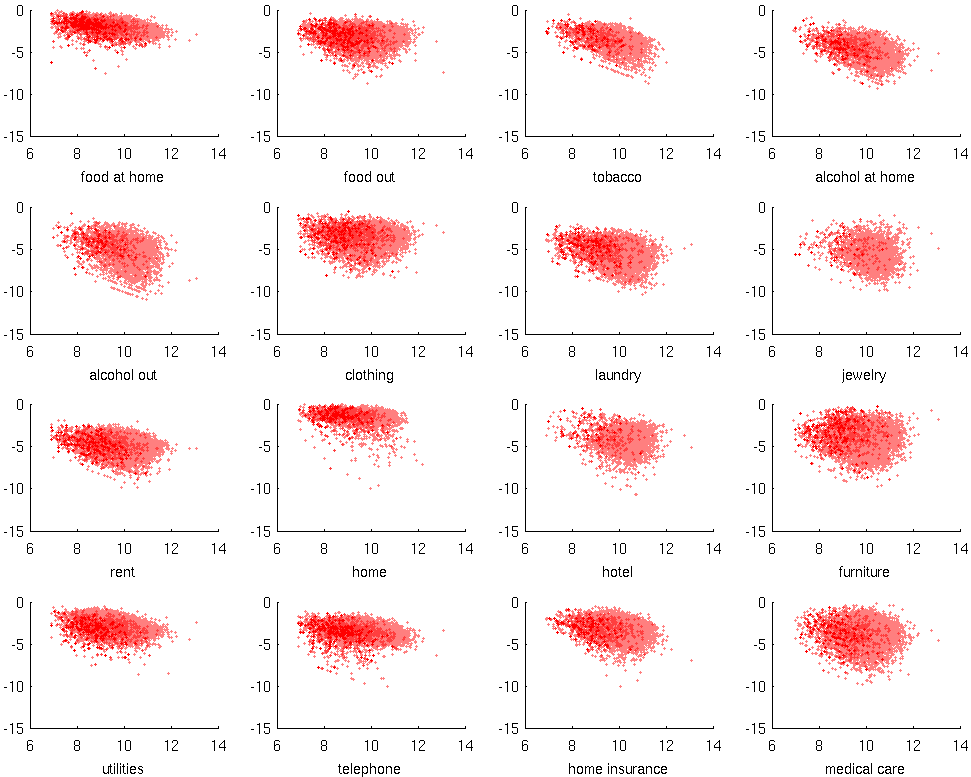
\includegraphics[scale=1]{pics/shares_cropped.pdf}
	\label{fig:shr}
	\caption{Log Expenditure Shares by Log Expenditure for select goods}
\end{figure}
\begin{figure}
	\centering
		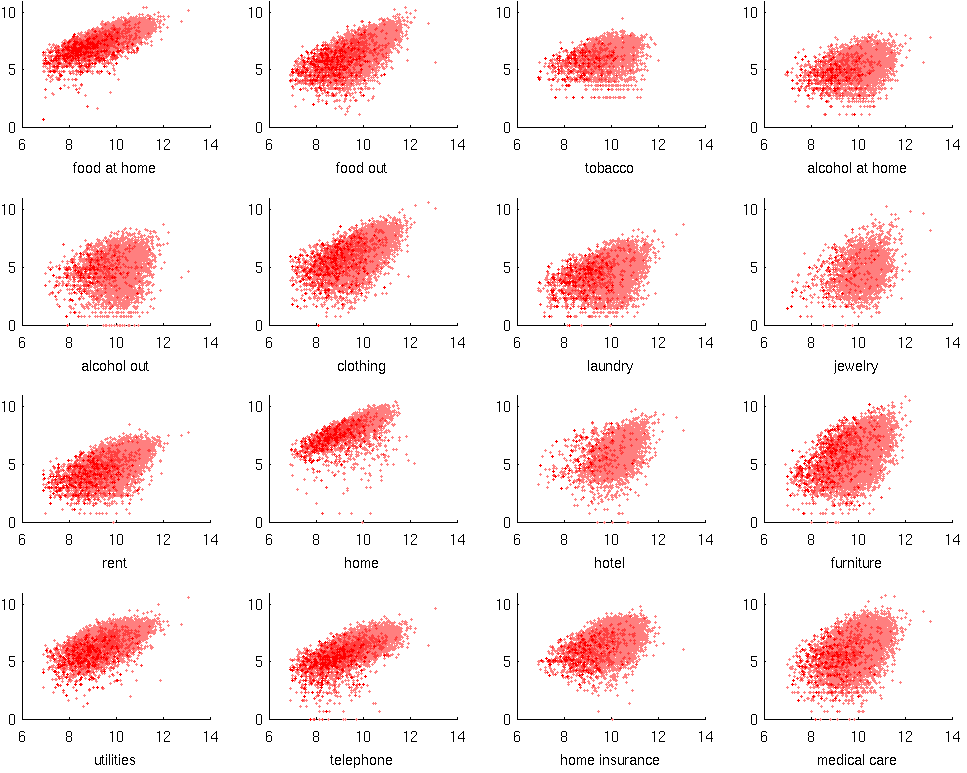
\includegraphics[scale=1]{pics/levels_cropped.pdf}
	\label{fig:lev}
	\caption{Log Category Expenditure by Log Expenditure for select goods}
\end{figure}
\begin{figure}
	\centering
		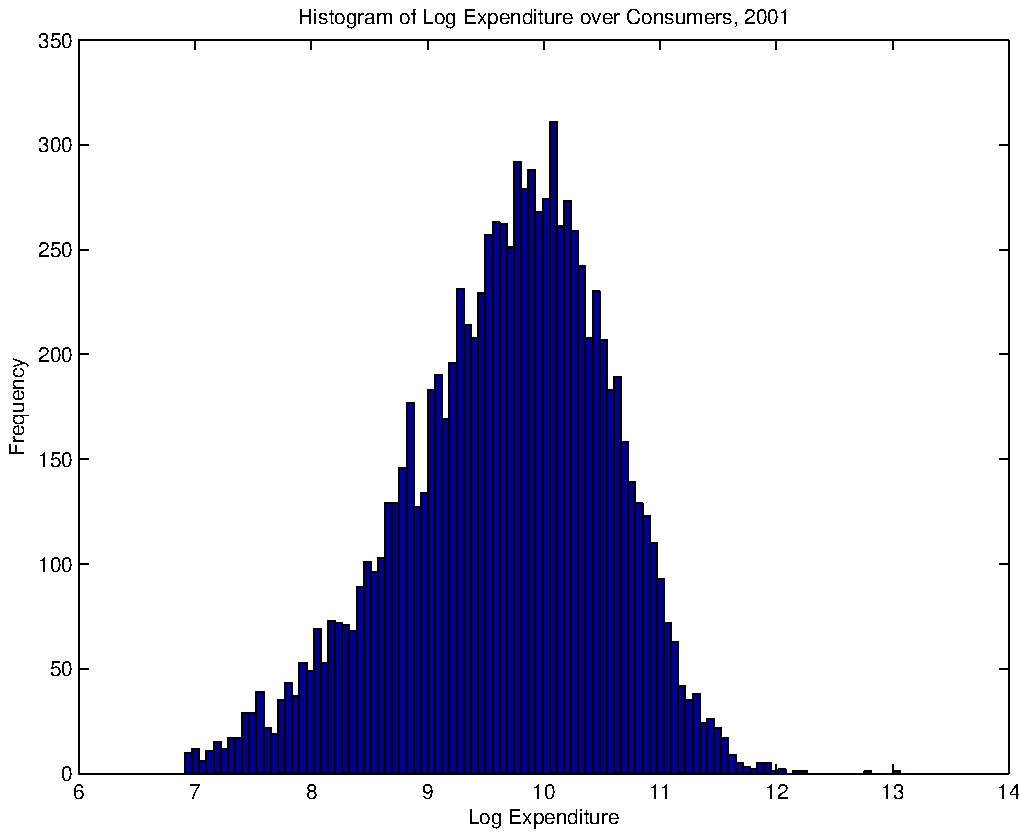
\includegraphics[scale=.8]{pics/exphist_cropped.pdf}
	\label{fig:exphist}
	\caption{Histogram of  Log Expenditure}
\end{figure}

For the Chinese household expenditures, I used publicly available data from the Chinese Household Income Project (CHIP) \citep{CHIP2002}. Like the American household expenditure data, the CHIP data comprises of repeated cross-sections of Chinese households.  In this study I use urban households surveyed in 1995 and 2002 for a total of 13,767 observations.  I use 14 good categories which correspond to aggregates of those in the American household expenditure survey.   The Table \ref{tab:chncons} describes how aggregation was done.  
\begin{table}
    \centering
    \footnotesize
    \begin{sideways}
	\begin{tabular}{|l|l|l|l|l|}
	    	\hline
		\textbf{US Cat}			 & \textbf{1995 Chn Cat}  & \textbf{2002 Chn Cat}  & \textbf{Chn Cat Name} & \textbf{Chn Price Name}\\
		\hline
		Fdh,Fdo	 		 & h27	 	 & e1-e152-e153	 & Food-Cig.-Alcohol	 		 	 & Food\\ 
		\hline
		Alh,Alo	 		 & h30-h31	 & e153	 	 & Alcohol	 				 & Liquor \& beverage\\
		\hline
		Cig	 		 & h31	 	 & e152	 	 & Cigarettes	 				 & Tobacco\\ 
		\hline
		Bks	 		 & h37	 	 & f631	 	 & Textbooks	 				 & Teaching mat. \& ref books\\ 
		\hline
		Edu	 		 & h38 to h42	 & f63-f631	 & Education-Textbooks	 	 		 & Education fares\\ 
		\hline
		Bus,Car*		 & h44	 	 & f514	 	 & Transportation	 			 & Transport. fares\\ 
		\hline
		Utl	 		 & h45 to h46	 & f72	 	 & Water, Elec., Fuel, \& other	 	 	 & Water, Elec., \& Fuel\\ 
		\hline
		Tel	 		 & h47	 	 & f522	 	 & Communication	 			 & Communication fares\\ 
		\hline
		Clo,Jwl	 		 & h32	 	 & f2 	  	 & Clothes	 				 & Clothing\\ 
		\hline
		Ot1,Ot2	 		 & h33	 	 & f6-f63	 & Entertain. \& Cultur. Serv.		 	 & Recreation fares\\ 
		\hline
		Fur,Lry,Brb	 	 & h34,h36	 & f3 	 	 & Home Equip., Facil., \& Serv.		 & Washing \& Haircut\\ 
		\hline
		Med,Lin	 		 & h48	 	 & f4 	 	 & Health \& Med. 			 	 & Medicine \& Med. serv.\\ 
		\hline
		Hom,Htl	 		 & h64	 	 & f71	 	 & Housing	 			 	 & Housing\\ 
		\hline
		Fee,Cha	 		 & h35	 	 & f8 	 	 & Misc. Goods \& Serv.			 	 & -\\ 
		\hline
	\end{tabular}
	\end{sideways}
    \caption{Chinese Consumption and Price Categories \scriptsize{*Air,Gas,Cmn,Cin}}
    \label{tab:chncons}
\end{table}

\subsection{Vindex}
Data about the relative visibility of  various types of goods is taken from \citet{Heffetz2011}.  
Heffetz bases the index on randomized telephone surveys conducted in the United States in several waves around 2004.
The main question of interest was about good categories.
Heffetz asked respondents how long it would take them to notice if a new acquaintance similar to themselves spent more than average on a particular good category.
Repondents were able to choose from five time periods ranging from almost immediately to almost never.  
Basic demographics were also recorded for respondents.  

From the survey responses, Heffetz creates indexes (called vindexes) between zero and one for each category of goods by averaging over survey results.  
A higher index implies that a good category is  more conspicuous. 
A result of this aggregation methodology is that the index is cardinal rather than ordinal.  Two goods with similar index values are similar in visibility.  Details on the implementation of the survey and calculation of the index are available in the original paper.
Table \ref{tab:vintab} below is an example of a vindex table for non-blacks under 40.
\begin{table}
    \centering
\begin{tabular}{|l|c|c|}
	\hline
	\textbf{Category} & \textbf{Vindex} & \textbf{SE} \\
	\hline
Clo (clothing) & 0.78 & (0.02)\\ 
	\hline
Cig (cigarettes) & 0.75 & (0.02)\\ 
	\hline
Car (cars) & 0.72 & (0.02)\\ 
	\hline
Fur (furniture) & 0.69 & (0.02)\\ 
	\hline
Ot1 (recreation 1) & 0.68 & (0.02)\\ 
	\hline
Jwl (jewelry) & 0.68 & (0.03)\\ 
	\hline
FdO (food out) & 0.67 & (0.02)\\ 
	\hline
AlH (alcohol home) & 0.66 & (0.03)\\ 
	\hline
AlO (alcohol out) & 0.65 & (0.02)\\ 
	\hline
Ot2 (recreation 2) & 0.61 & (0.02)\\ 
	\hline
Brb (barbers etc) & 0.6 & (0.03)\\ 
	\hline
Bks (books etc) & 0.58 & (0.02)\\ 
	\hline
Edu (education) & 0.55 & (0.03)\\ 
	\hline
Hom (rent/home) & 0.54 & (0.03)\\ 
	\hline
FdH (food home) & 0.51 & (0.03)\\ 
	\hline
Cel (cell phone) & 0.47 & (0.03)\\ 
	\hline
Htl (hotels etc) & 0.46 & (0.02)\\ 
	\hline
Air (air travel) & 0.44 & (0.03)\\ 
	\hline
Bus (public trans.) & 0.44 & (0.03)\\ 
	\hline
CMn (car repair) & 0.38 & (0.03)\\ 
	\hline
Cha (charities) & 0.36 & (0.03)\\ 
	\hline
Gas (gasoline) & 0.34 & (0.03)\\ 
	\hline
Lry (laundry) & 0.32 & (0.03)\\ 
	\hline
Med (health care) & 0.32 & (0.02)\\ 
	\hline
Tel (home phone) & 0.25 & (0.03)\\ 
	\hline
Utl (home utilities) & 0.25 & (0.03)\\ 
	\hline
Fee (legal fees) & 0.24 & (0.02)\\ 
	\hline
CIn (car insur.) & 0.22 & (0.03)\\ 
	\hline
LIn (life insur.) & 0.15 & (0.02)\\ 
	\hline
Und (underwear) & 0.14 & (0.02)\\ 
	\hline
HIn (home insur.) & 0.13 & (0.02)\\ 
	\hline
\end{tabular}
\label{tab:vintab}
\caption{Vindex for non-blacks under 40.}
\vspace{-2in}
\end{table}
I do not have a vindex equilivalent for Chinese people, so I just use the overall American vindex data for the Chinese estimation. Since there are fewer good categories in the Chinese data, I aggregate the vindex by taking the mean over the aggregated good categories. 
\subsection{Prices}
I have a time-series of relative price data from the Bureau of Labor services.
Most of the NBER household good categories were easy to match with the definitions used by the BLS.   
Since prices are normalized to one in 1983, the units of each good which enter into the utility function are whatever one dollar could buy in 1983.
The following page is a table showing the price category names I used compared with the NBER good categories:
    \begin{table}
	\footnotesize
	\centering
\begin{sideways}
\begin{tabular}{|l|l|l|}
\hline
VinCat Abrev & Vindex Category & PriceCatName\\ 
\hline
Brb & barbershops, beauty parlors, hair dresser, health clubs, etc. & Personal Care Services\\ 
\hline
Clo & clothing and shoes, not including underwear, undergarments and nightwear & Apparel\\ 
\hline
Cig & tobacco products like cigarettes, cigars, and pipe tobacco & Tobacco and Smoking Products\\ 
\hline
Jwl & jewelry and watches & Jewelry and watches\\ 
\hline
Car & the purchase of new and used motor vehicles such as cars, trucks, and vans & New and used motor vehicles\\ 
\hline
FdO & dining out at restaurants, drive-thrus, etc, exl. Alcohol incl. Food at school & Food away from home\\ 
\hline
Ot1 & computers, games, TVs, video, audio, musical and sports equipment, tapes, CDs. & Televisions\\ 
\hline
FdH & food and nonalcoholic beverages at grocery, specialty and convenience stores. & Food at home\\ 
\hline
Edu & education, from nursery to college, like tuition and other school expenses. & Tuition, other school fees, and childcare\\ 
\hline
Cel & mobile phone services. & Wireless Telephone Services\\ 
\hline
AlO & alcoholic beverages at restaurants, bars, cafeterias, cafes, etc. & Alcoholic Beverages away from home\\ 
\hline
AlH & alcoholic beverages for home use. & Alcoholic Beverages at home\\ 
\hline
Fur & home furnishings and household items, like furniture, appliances, tools, linen. & Furniture and bedding\\ 
\hline
Ot2 & cable TV, pets and veterinarians, sports, country clubs, movies, and concerts. & Cable and satellite television\\ 
\hline
Bks & books incl. School books, newspapers and magazines, toys, games, and hobbies. & Recreational reading materials\\ 
\hline
Cmn & vehicle maintenance, mechanical and electrical repair and replacement. & Motor vehicle maintainance\\ 
\hline
Hom & rent, or mortgage, or purchase, of housing & Housing\\ 
\hline
Htl & lodging away from home on trips, and housing for someone away at school. & other lodging away from home\\ 
\hline
Bus & public transportation, both local and long distance, like busses and trains. & Public transportation\\ 
\hline
Air & airline fares for out-of-town trips. & Airline Fare\\ 
\hline
Gas & gasoline and diesel fuel for motor vehicles. & Motor Fuel\\ 
\hline
Tel & home telephone services, not including mobile phones. & Telephone Services\\ 
\hline
Cha & contributions to churches or other religious organizations, and other charities. & Missing\\ 
\hline
Lry & laundry and dry cleaning. & Laundry equipment\\ 
\hline
Utl & home utilities such as electricity, gas, and water, garbage collection. & Fuel and Utilities\\ 
\hline
Med & medical care, incl. Health insurance, drugs, dentists, doctors, hospitals, etc. & Medical care\\ 
\hline
Fee & legal fees, accounting fees, and occupational expenses like tools and licenses. & Professional services\\ 
\hline
Cin & vehicle insurance, like insurance for cars, trucks, and vans. & Motor vehicle insurance\\ 
\hline
Hin & homeowners insurance, fire insurance, and property insurance. & Tenants' and household insurance\\ 
\hline
Lin & life insurance, endowment, annuities, and other death-benefits insurance. & Health insurance\\ 
\hline
\end{tabular}
\end{sideways}
\end{table}
Chinese prices are taken from the China Statistical Yearbook (\citep{CSY}).  The Chinese prices are denominated in Renminbi, and are normalized to one in 1995--my first year of data. The Chinese price category comparison is located in Table \ref{tab:chncons}. 

\section{Estimation}
\subsection{Specializing to Cobb-Douglas}

Let the fundamental utility function be Cobb-Douglas:
\[u(\mathbf{C}) = \sum_{g=1}^{G} \gamma_g \ln(c_g)\]
The model can then be written as a generalization of the Heffetz model to many goods and preference heterogeneity.\footnote{ In the Heffetz version, there are only two goods, one visible and the other invisible to society. In my version, there is one visible good for each observation type, and all the other goods are invisible.}
In what follows I drop subscripts for Consumer $i$ to simplify notation. Let $t \in G$ be Consumer $i$'s observation type, and let $c_{t}^*$ be Consumer $i$'s equilibrium consumption of the visible good.  Equilibrium demand for good $g\neq t$ conditional on spending on the visible good is the standard Cobb-Douglas constant expenditure share:
\[p_g c_g^* = \gamma_g\left(\sum_{j\neq t} \gamma_j\right)^{-1}\left(w-p_t c_t^* \right)\]

Using the demands, we can write the utility function as a function of visible good consumption.
\begin{equation}
    \label{eq:ufun}
    U(c_t) = (1-\alpha) \left(\hat{\gamma} \ln \left(w-p_t c_t\right) + \gamma_t \ln \left(c_t \right)\right) + \alpha \left(\gamma_t \ln \left(s(c_t)\right) + \gamma_t \ln \left(c_t\right) \right) + \zeta(\mathbf{p},\mathbf{\gamma})
\end{equation}
Here $\hat{\gamma} = \sum_{g\neq t} \gamma_g$ and $\zeta(\mathbf{p},\mathbf{\gamma})$ is a constant which depends only on utility parameters and prices.  The single-valued function $s(c_t)$ is the belief of the peer group about spending on non-visible goods $w-p_t c_t$. 

Consumer $i$ maximizes utility function \eqref{eq:ufun} subject to his budget constraint.  The first order condition for an interior solution to his problem can be written:
\begin{equation}
	\label{foc}
s'(c_t^*) = \frac{1}{\alpha}\left( \left( 1-\alpha\right) p_t - \frac{\gamma_t}{\hat{\gamma}}\frac{s(c_t^*)}{c_t^*}\right)
\end{equation}
This differential equation has the solution:
% Now we can directly follow Heffetz and solve this differential equation:
% \begin{equation}
% 	\label{difsol}
% 	s(c_t^*) = \frac{\hat{\gamma}\left(1-\alpha\right)}{\gamma_t +\alpha \hat{\gamma}} p_t c_t + K c_t^{-\frac{\gamma_t}{\alpha \hat{\gamma}}}
% \end{equation}
% To solve for the constant $K$, we use the idea that the lowest possible wealth type $\underbar{W}$ has no reason to signal in a separating equilibrium.
% From his perspective, things are already as bad as they can be, so there is no reason for him to distort his consumption to signal.  His demand $\underbar{c}$ for $c_t$ will be given by:
% \begin{equation}
% 	\label{lowc}
% 	\underbar{c} = \frac{\gamma_t}{p_t}\left(\sum_{j} \gamma_j\right)^{-1}\underbar{W} 
% \end{equation}
% Since in equilibrium $s(\underbar{c}) = \underbar{W} - p_t \underbar{c}$, we can plug into \eqref{difsol} and solve for $K$:
% \[
% K = \frac{\underbar{W}- \frac{\gamma_t + \hat{\gamma}}{\gamma_t + \alpha \hat{\gamma}}p_t \underbar{c}}{\underbar{c}^{-\frac{\gamma_t}{\alpha \hat{\gamma}}}}
% \]
\begin{equation}
	\label{eq:difsol}
    s(c_t^*) = \frac{\hat{\gamma}\left(1-\alpha\right)}{\gamma_t +\alpha \hat{\gamma}} p_t c_t^* +  \frac{\hat{\gamma} \alpha }{\gamma_t + \alpha \hat{\gamma}} \underbar{W}\frac{p_t c_t^*}{p_t \underbar{c}}^{-\frac{\gamma_t}{\alpha \hat{\gamma}}}
\end{equation}
The constant in the solution \eqref{eq:difsol} is pinned down by the fact that the lowest possible wealth type $\underbar{W}$ has no reason to signal in a separating equilibrium.  His expenditure on the visible good $\underbar{c}$ is the fraction $\frac{\gamma_t}{\sum_j \gamma_j}$ of his wealth.  As one might expect, the function $s$ is jointly homothetic in $c_t$ and $\underbar{W}$.
\footnote{
Below I show that $s$ is jointly homothetic of degree one in $\underbar{W}$ and $c_t$.  First, it is immediate from \eqref{lowc} that $\underbar{c}$ scales linearly with $\underbar{W}$.
Now $K$ scales non-linearly with $\underbar{W}$:
\begin{align*}
	K(\xi\underbar{W}) &= \frac{\xi\underbar{W}- \frac{\gamma_t + \hat{\gamma}}{\gamma_t + \alpha \hat{\gamma}}p_t \xi \underbar{c}}{(\xi\underbar{c})^{-\frac{\gamma_t}{\alpha \hat{\gamma}}}} \\
	&= \xi^{1 + \frac{\gamma_t}{\alpha \hat{\gamma}}}K(\underbar{W})
\end{align*}
The way $K$ scales, however, is just right to make $s$ scale linearly in $c_t$:
\begin{align*}
	s(\xi c_t,\underbar{W}) &= \frac{\hat{\gamma}\left(1-\alpha\right)}{\gamma_t +\alpha \hat{\gamma}} p_t \xi c_t + \xi^{1+\frac{\gamma_t}{\alpha \hat{\gamma}}} K(\underbar{w}) (\xi c_t)^{-\frac{\gamma_t}{\alpha \hat{\gamma}}} \\
	&= \frac{\hat{\gamma}\left(1-\alpha\right)}{\gamma_t +\alpha \hat{\gamma}} p_t \xi c_t + \xi K(\underbar{w}) c_t^{-\frac{\gamma_t}{\alpha \hat{\gamma}}} \\
	&= \xi s(c_t,\underbar{W})
\end{align*}

If $c^*$ is an interior maximizer of \eqref{ufun} for an individual of wealth $W$, then $\xi c^*$ is a solution to the  problem of an individual of wealth $\xi W$, as long as we also scale $\underbar{W}$ up by $\xi$ as well.
If $c^*$ is an interior maximizer, then it solves the first order conditions of \eqref{ufun}:
\[
\frac{(1-\alpha)r_v \hat{\gamma}}{W-r_v c^*} = \frac{\alpha \gamma_v s'(c^*)}{s(c^*)} + \frac{\gamma_v}{c^*}
\]
Now divide both sides of the equation by $\xi$, and using the fact that $s$ is homothetic of degree one and $s'$ is homothetic of degree zero, we get:
\[
\frac{(1-\alpha)r_v \hat{\gamma}}{\xi W-r_v \xi c^*} = \frac{\alpha \gamma_v s'(\xi c^*)}{s(\xi c^*)} + \frac{\gamma_v}{\xi c^*}
\]
Thus, $\xi c^*$ solves the scaled problem.
}

Define equilibrium expenditure share on the visible good category $r = p_t c_t^* / w$, the ratio $\gamma = \gamma_t / \hat{\gamma}$, and the ratio of minimum wealth to own wealth $\hat{w} = \underbar{W} / w$.  Substituting in for the $s$ function and dividing by wealth, we have a simplified equilibrium condition:

\begin{equation}
	\label{eq:eq_cond}
    (1 - r)(1 + \frac{\gamma}{\alpha}) = \frac{\left(1-\alpha\right)}{\alpha} r +  \left(r\left(1 + \gamma^{-1}\right)\right)^{-\frac{\gamma}{\alpha}}\hat{w}^{1+\frac{\gamma}{\alpha}}
\end{equation}

\subsection{Estimation Equations}
We are interested in $\alpha$, the weight given to the peer-belief part of the utility function.  In order to estimate $\alpha$, we must jointly estimate the observation type of each household.  I use a two step 'hard' expectation maximization algorithm.  In the first stage, I condition on the observation type of each household and update $\alpha$ and preference parameter distributions.  In the second stage, I take $\alpha$ and the preference parameter distributions as given and find the most likely observation type of each household.  The algorithm stops when there is nearly no change in $\alpha$.

\subsection{Likelihood function}

Given consumption, household utility parameters $\gamma(\alpha,t_i|C_i)$ are a function of the utilty weight $\alpha$ and the observation type $t_i$.  Consider a household of wealth type $w$ and with consumption vector $C$.  Suppose that the household is observation type $t$.
Then the consumptions of goods $j\neq t$ are given by:
\begin{align}
	\label{eq:sgd}
	p_jc_j &= \frac{\gamma_j}{\sum_{g\neq t}\gamma_g}  \left(w-  p_t c_t\right)\\
	\label{eq:sgdsol}
	\gamma_j &= \frac{p_j c_j}{\left(w- p_t c_t\right)} \sum_{g\neq t}\gamma_g  
\end{align}

We can solve for the 28 non-observation type $\gamma$'s up to a scaling factor $\sum_{g\neq t}\gamma_g$.
I normalize the parameter $\gamma_1$ on consumption of food at home to one. 
\footnote{It is important to choose a good which always has positive consumption, since this strategy will not work if consumption of the normalized good is zero.  
Food at home is consumed in all but 800 of the 150,000 US households.}

If food at home is not the observation type, then 
\begin{equation}
	\label{eq:gamsol}
	\gamma_j = \frac{p_j c_j}{p_1 c_1}
\end{equation}
Using \eqref{eq:gamsol} and \eqref{foc}, $\gamma_t$ can be written as:
\begin{equation}
    \label{eq:exact_gt}
    \gamma_t = \hat{\gamma} \frac{r - \alpha}{1 - r} + \hat{\gamma}\frac{\alpha}{\ln \tilde{c}} W\left(\frac{\tilde{w} \tilde{c}^{\frac{a - r}{a(1 - r)}}\ln \tilde{c}}{1 - r}\right)
\end{equation}
Here $\tilde{c} = p_t c_t / p_t \underbar{c}$ and $\tilde{w} = w / \underbar{W}$. The large $W$ function is the Lambert W Function.  Unfortunately, \eqref{eq:exact_gt} is not closed form, as $\tilde{c}$ is not observed and depends upon $\gamma_t$.

Let $\mu$ and $\sigma$ be vectors of log-normal location and dispersion parameters, and let $z$ be a vector of zero probabilities. Let $\phi$ be the log-normal probability density function. Let household $h$'s preference parameter for good $g$, which is a function of $\alpha$, be $\gamma_{hg}(\alpha)$.  The likelihood function is:
\begin{equation}
	\label{lik1}
    \sum_{i}\left[ \ln(v^i_{t_i}) + \sum_{g} \left(\mathbf{1}_{\{\gamma_{hg}(\alpha, t_i) = 0\}}\ln\left(z_g\right) + \mathbf{1}_{\{\gamma_{hg}(\alpha, t_i) \neq 0\}} \left(\ln\left(1 - z_g\right)+\ln \phi(\gamma_{hg}(\alpha, t_i)|\mu_g,\sigma_g)\right)\right)\right]
\end{equation}

\subsection{Nuisance parameter maximization}

Given a utility weight $\alpha$ and a set of preference distribution parameters, we need to choose the most likely observation type for each household. Let P is the vector of vindex probabilities.  $\gamma_{hi}$ remains an implicit function as in \eqref{lik1} above:
\begin{equation}
    \label{lik2}
    l_h^2(i) = \ln(p_i) + \sum_{i} \left(\mathbf{1}_{\{\gamma_{hi} = 0\}}\ln\left(z_i\right) + \mathbf{1}_{\{\gamma_{hi} \neq 0\}} \left(\ln\left(1-z_i\right)+\ln \phi(\gamma_{hi}|\mu_i,\sigma_i)\right)\right)
\end{equation}
In practice, in the United States I have different visibility indexes for four groups of households: blacks under 40, blacks over 40, non-blacks under 40, and non-blacks over 40.
The vector $P$ will differ for these different demographic groups.
The visibility probabilities are taken directly from Heffetz and normalized so that they sum to one.
\footnote{A household is identified by the self-identified characteristics of whoever answered the consumption survey. 
In a previous version of this project, I needed to calculate equilibrium consumptions for each type.  This led me to keep the type nmber small.  In the current version, the number of types does not affect the speed of estimation.  Another extension would be to increase the types to the maximum number allowed by the Heffetz survey. This would help with identification.}

In the American data, $\mu$ , $\sigma$, and $z$ are each 28 dimensional vectors. Adding $\alpha$ gives us a total of 85 parameters to be estimated in the first stage.   
In my useable dataset, I have 154,016 households which is 1,800 household observations per parameter.
However, to save computation time, I am currently using only 10,000 randomly-chosen household observations, or a little over 100 observations per parameter.
The Chinese version of the model, the preference heterogeneity vectors are only 13 dimensions, so there are 40 parameters to be estimated.  My baseline Chinese estimate is done using 5000 randomly-chosen households, so again there are a little over 100 households per parameter.
Since the preference heterogeneity is assumed to be independent, given observation types and an $\alpha$ I can use the (log) sample mean and variance to recover the likelihood maximizing $z$, $\mu$, and $\sigma$'s.
Thus the numerical part of the maximization step above is really only over the single dimensional $\alpha$ parameter.
\subsection{Identification}
We can think of identification separately in the two stages of the EM estimation described above.  In the second stage, observation type is identified by abnormally large expenditures in a single good category.  Cigarettes are a great example.  Most households spend a very small amount on tobacco products.  Some households, however, spend a very large amount.  As will be seen in the results section below, this leads to many assignments of cigarettes to observation type.  The same is true of jewelry and education.

In the first stage, while  I restrict all residents of a single country to share the same fundamental utility functional form, I allow vindex probabilities to differ across sub-populations.  Thus, if the data show that, say, blacks under 40 have significantly different consumption patterns (on average) compared with non-blacks under 40, the estimation will chalk it up to differences in the visibility of goods, which will lead to a large $\alpha$.  The more demographic categories I have and the more variation there is in average consumption between demographics, the better will this identification strategy work. 

Since in China I currently have a single demographic category, the identification is going to be purely off of the functional form.  In particular, since fundamental utility is Cobb-Douglas, more curvy average Engel curves will result in larger $\alpha$'s.
\section{Results}
Tables \ref{tab:parest} and \ref{tab:chnparest} below respectively present American and Chinese parameter estimates.  
The standard errors in the tables should be regarded somewhat cautiously, as these are done using the Fisher information from the first-stage likelihood alone.  In essence, they are the standard errors assuming that the observation types are known.  The proper way to get the standard errors would be to bootstrap.  The optimization routine is currently quite slow, however, and I have not done this yet.
\begin{table}
	/centering
		\begin{tabular}{|l|c c |c c |c c|}
			\hline
			Good Cat & $\mu$ & std err      & $\sigma$ & std err       & $pr(\gamma_j =  0)$ & std err\\
			\hline
			FdO & -1.2106 &  (0.0002) &  1.1823 & (0.0005) &   0.0836 & (0.0038)\\ 
			\hline
			Cig & -6.1907 &  (0.0022) & 11.4001 & (0.0512) &   0.8274 & (0.0054)\\ 
			\hline
			AlH & -2.7418 &  (0.0002) &  1.2418 & (0.0006) &   0.4760 & (0.0070)\\ 
			\hline
			AlO & -3.0832 &  (0.0003) &  1.6011 & (0.0010) &   0.5032 & (0.0070)\\ 
			\hline
			Clo & -1.4358 &  (0.0002) &  1.1580 & (0.0005) &   0.0938 & (0.0040)\\ 
			\hline
			Lry & -3.3559 &  (0.0002) &  1.3826 & (0.0007) &   0.3102 & (0.0065)\\ 
			\hline
			Jwl & -5.3608 &  (0.0015) &  8.1810 & (0.0228) &   0.6604 & (0.0067)\\ 
			\hline
			Brb & -2.6958 &  (0.0002) &  1.0096 & (0.0004) &   0.1530 & (0.0050)\\ 
			\hline
			Hom &  0.3824 &  (0.0002) &  0.8689 & (0.0004) &   0.7046 & (0.0065)\\ 
			\hline
			Htl & -2.4135 &  (0.0002) &  1.3596 & (0.0007) &   0.6360 & (0.0068)\\ 
			\hline
			Fur & -1.9858 &  (0.0002) &  1.4964 & (0.0008) &   0.2570 & (0.0061)\\ 
			\hline
			Utl & -0.8731 &  (0.0001) &  0.7561 & (0.0002) &   0.0960 & (0.0041)\\ 
			\hline
			Tel & -1.6308 &  (0.0001) &  0.9058 & (0.0003) &   0.0360 & (0.0025)\\ 
			\hline
			HIn & -1.5132 &  (0.0002) &  1.1389 & (0.0005) &   0.4102 & (0.0069)\\ 
			\hline
			Med & -1.8537 &  (0.0002) &  1.3468 & (0.0007) &   0.2514 & (0.0061)\\ 
			\hline
			Fee & -2.9173 &  (0.0002) &  1.3449 & (0.0007) &   0.3530 & (0.0067)\\ 
			\hline
			LIn & -2.2290 &  (0.0002) &  1.2182 & (0.0006) &   0.5192 & (0.0070)\\ 
			\hline
			Car & -2.3967 &  (0.0003) &  1.8427 & (0.0013) &   0.5890 & (0.0069)\\ 
			\hline
			CMn & -2.2251 &  (0.0003) &  1.5484 & (0.0009) &   0.2236 & (0.0058)\\ 
			\hline
			Gas & -1.0737 &  (0.0001) &  0.8481 & (0.0003) &   0.0956 & (0.0040)\\ 
			\hline
			CIn & -1.4963 &  (0.0001) &  0.8789 & (0.0003) &   0.3360 & (0.0066)\\ 
			\hline
			Bus & -6.1303 &  (0.0014) &  8.6399 & (0.0211) &   0.7626 & (0.0060)\\ 
			\hline
			Air & -2.2693 &  (0.0003) &  1.6096 & (0.0010) &   0.6914 & (0.0065)\\ 
			\hline
			Bks & -3.4553 &  (0.0002) &  1.4929 & (0.0008) &   0.4718 & (0.0070)\\ 
			\hline
			Ot1 & -2.7484 &  (0.0002) &  1.1775 & (0.0005) &   0.1316 & (0.0047)\\ 
			\hline
			Ot2 & -1.3021 &  (0.0002) &  1.2837 & (0.0006) &   0.0828 & (0.0038)\\ 
			\hline
			Edu & -5.8550 &  (0.0019) & 10.3474 & (0.0383) &   0.8262 & (0.0054)\\ 
			\hline
			Cha & -2.3950 &  (0.0003) &  1.5843 & (0.0010) &   0.5950 & (0.0069)\\ 
			\hline
		        \hline	
			$\alpha$ & 0.1459 & (0.0071) & & & & \\
			\hline
			\hline
		\end{tabular}
	\caption{US Parameter Estimates}
	\label{tab:parest}
\end{table}
\begin{table}
    \centering
	\begin{tabular}{|l|c c |c c |c c|}
		\hline
		Good Cat & $\mu$ & std err      & $\sigma$ & std err       & $pr(\gamma_j =  0)$ & std err\\
		\hline
		Cig         & -6.4154 &  (0.1116) & 5.6359 & (0.8895) & 0.4845 & (0.0070)\\ 
		\hline
		Alo/Alh     & -9.0358 &  (0.0778) & 5.1898 & (0.5713) & 0.1014 & (0.0042)\\ 
		\hline
		Clo/Jwl     & -1.5462 &  (0.0134) & 0.9407 & (0.0178) & 0.0109 & (0.0014)\\ 
		\hline
		Ot1/Ot2     & -2.5040 &  (0.0227) & 1.5752 & (0.0507) & 0.0339 & (0.0025)\\ 
		\hline
		Fur/Lry* & -2.5019 &  (0.0202) & 1.3996 & (0.0400) & 0.0325 & (0.0024)\\ 
		\hline
		Med/Lin     & -5.1053 &  (0.0714) & 4.8383 & (0.4887) & 0.0725 & (0.0036)\\ 
		\hline
		Bus/Car* & -3.7775 &  (0.0226) & 1.4489 & (0.0464) & 0.1722 & (0.0053)\\ 
		\hline
		Tel         & -10.477 &  (0.1173) & 6.8838 & (1.1426) & 0.3046 & (0.0064)\\ 
		\hline
		Edu         & -2.0158 &  (0.0211) & 1.2802 & (0.0382) & 0.2565 & (0.0061)\\ 
		\hline
		Bks         & -4.3451 &  (0.0357) & 1.6896 & (0.0854) & 0.5490 & (0.0070)\\ 
		\hline
		Hom/Htl     & -5.5897 &  (0.0620) & 3.0517 & (0.2677) & 0.5108 & (0.0070)\\ 
		\hline
		Utl         & -2.3232 &  (0.0113) & 0.7959 & (0.0128) & 0.0135 & (0.0016)\\ 
		\hline
		Fee/Cha     & -2.2273 &  (0.0180) & 1.2589 & (0.0321) & 0.0167 & (0.0018)\\ 
		\hline
	        \hline	
		$\alpha$ & 0.2618 & (0.0002) & & & & \\
		\hline
	\end{tabular}
     	\linebreak
	\small{*Fur/Lry/Brb, Bus/Car/Gas/Air/Cmn/Cin}
    \caption{Chinese Parameter Estimates}
    \label{tab:chnparest}
\end{table}
The main parameter of interest, the weight of conspicuous consumption in utility, is 0.1459 and 0.2618 in the US and China respectively.  This means that one util of peer group belief is worth $0.1459/(1-0.1456) \approx 17\%$ as much as a util of fundamental utility in the United States.  In China this number is $0.2618/(1-0.2618) \approx 35\%$.  According to the estimated parameters, Chinese people weight peer group belief twice as heavily as Americans do.

The model does a good job of simulating data similar to the real data set. In Figure \ref{fig:shares_fake} and figure \ref{fig:levels_fake} are scatter plots of simulated US data, made in the same way as the scatter plots of the actual US data in figures \ref{fig:shr} and \ref{fig:lev}. 
\begin{figure}
	\centering
		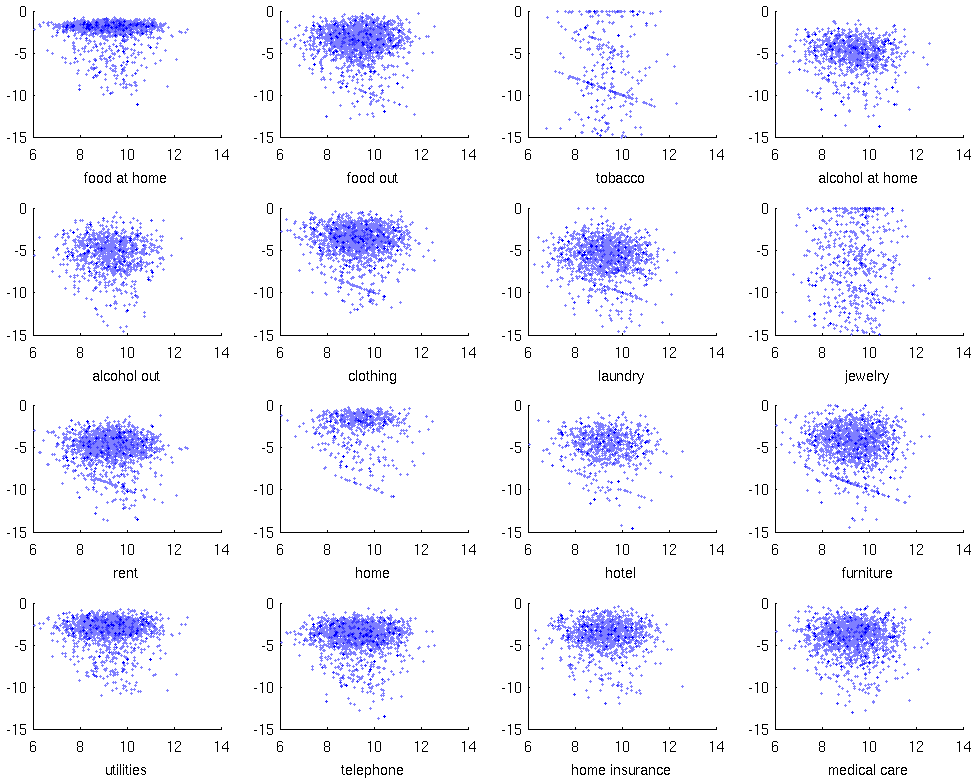
\includegraphics[scale=1]{pics/shares_fake_cropped.pdf}
	\caption{Simulated expenditure share plots by category.}
	\label{fig:shares_fake}
\end{figure}
\begin{figure}
    \centering
	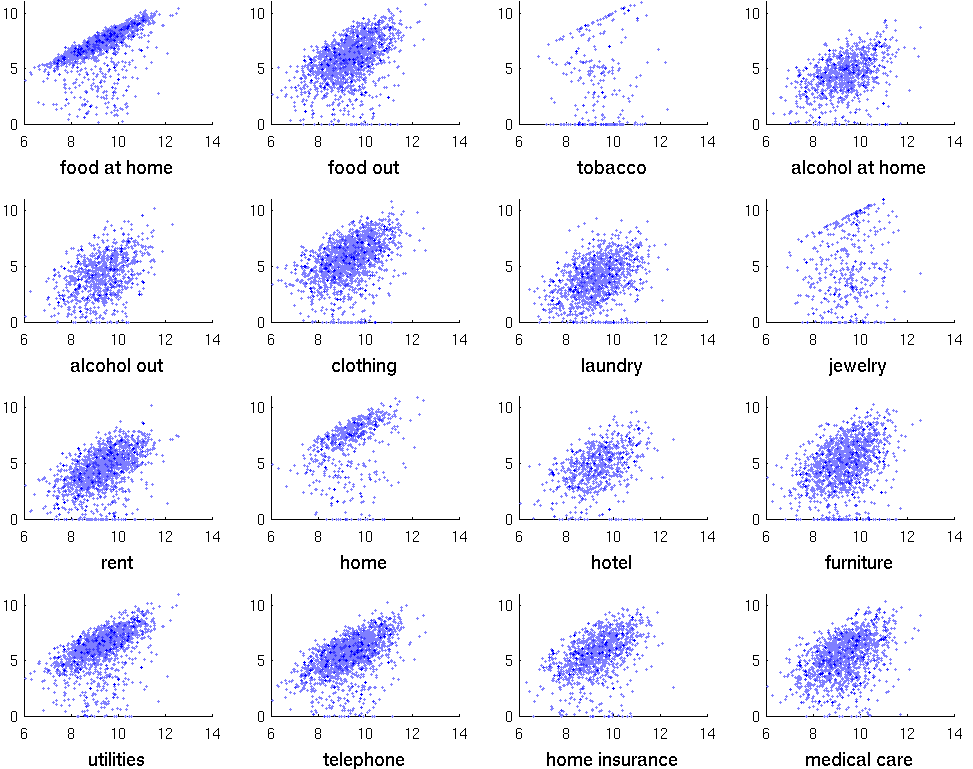
\includegraphics[scale=1]{pics/levels_fake_cropped.pdf}
    \caption{Simulated expenditure level plots by category.}
    \label{fig:levels_fake}
\end{figure}
The simulated data only have 5000 observations compared with the full dataset's upwards of 150,000 observations. 
Besides the sparcity, however, the simulated data qualitatively do a good job recreating the real world data.

The estimation does less well on observation types.
Ideally the observation type distribution (for a particular demographic) should be the same as the vindex probability distribution from the Heffetz survey.
The estimated American observation type densities, however, have only a $0.3778$ correlation with the vindex probabilities.
Figure \ref{fig:vinmatch} is a scatter plot of the vindex probabilities and the estimated observation type densities.
\begin{figure}
    \centering
	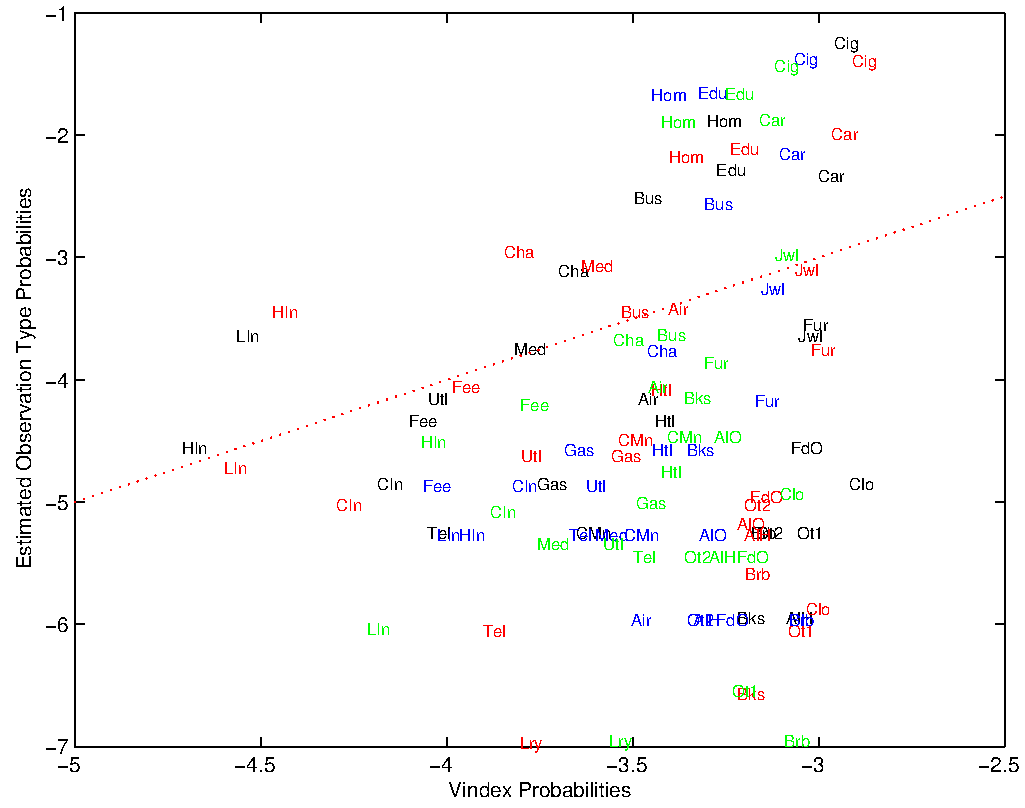
\includegraphics[scale=.8]{pics/vinmatch_cropped.pdf}
    \caption{Estimated (log) observation type distribution compared to (log) Heffetz vindex.}
    \label{fig:vinmatch}
\end{figure}
Each point is labeled with the relevant good category, and the colors represent different demographic types (black or not, under or over 40).
The estimated probabilities are exagerated compared with the vindex probabilities.

\subsection{Tax on automobile purchases}

Automobiles are one of the most visible good categories. In this section, I consider the welfare gains from a sales tax on automobiles, redistributed lumpsum as a fraction of wealth.  When redistributed this way, taxes will not cause a change in either the individual or aggregate fraction of wealth allocated to any particular good category, as relative wealth remains unchanged.  
An automobile sales tax will increase the utility of a consumer by scaling consumption of all non-automobile goods up, but will lower utility by reducing automobile consumption.  The net effect of the tax is indeterminate, and I numerically solve the model to find the optimal sales tax for an equally weighted social welfare function.

In the United States, taxes on blah.  I use the price level in 1980 as my baseline, and evaluate how close the current tobacco tax is to the estimated optimum.

Let $s$ be the share of aggregate wealth spent on automobiles.  If a fraction $u$ of spending on automobiles is taxed, the resulting revenue will be $su / (1 - su)$ multiplied by aggregate wealth.  Consumption of non-automobile goods will be $1 / (1-su)$ multiplied by pre-tax consumption levels, and consumption of automobiles will be $(1 - u) / (1 - su)$ multiplied by pre-tax automobile consumption.

Let $s_i$ be the share of consumer $i$'s endowment spent on automobiles.  To find the optimal tax, I numerically solve the following problem for the households in my sample:

\begin{equation}
    \underset{u}{\arg \max} \sum_i \left(\sum_{g \neq \mbox{\tiny{aut}}} \gamma_{gi} \ln \frac{s u}{1-s u} + \gamma_{\mbox{\tiny{aut, i}}} \ln \frac{1-u}{1 - s u}\right)
\end{equation}













Now that we have an estimated model, we can talk about the welfare costs of signaling.
The counterfactual exercise I conduct in this section is to set $\alpha$ to zero and track the increase in utility for various observation types.
In this section, as well as the tax section which follows, I focus on the American data.  Since the Chinese care more about peer group beliefs, these results apply a fortiori to the Chinese case.

Consider a typical consumer (with the modal preference parameter for each category) of various wealth levels.  
Figure \ref{fig:uchnge} plots percentage gain in utility after setting $\alpha = 0$ over expenditures (from 1000-20,000 dollars a year) for the 28  observation types.
I broke out housing because the welfare gain is much higher than in the other observation types.
As we would  predict, the wealthier a household is, the more it has to gain from eliminating signaling.
This is because wealthier households need to distort their consumption more to signal their wealth. 
Note that the poorest households gain nothing from an elimination of signaling, since they hardly signal anyway.

\begin{figure}
    \centering
	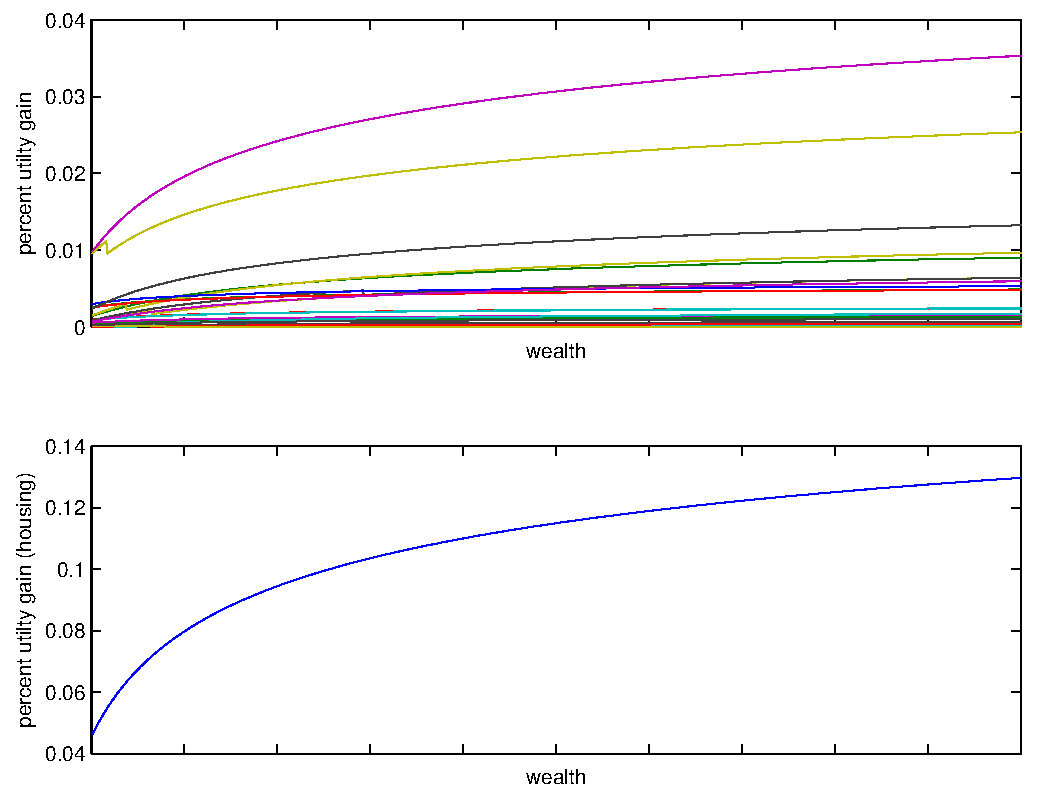
\includegraphics[scale=.8]{pics/uchnge_cropped.pdf}
    \caption{Percentage welfare gain due to the elimination of signaling, by observation type}
    \label{fig:uchnge}
\end{figure}
What I want the reader to take from this figure is that signaling behavior carries a real welfare cost.  For peer groups which signal with housing, this can be as much as 5\% of total utility.  Of course, policy cannot change people's preferences.  The next section examines a tax policy which has the potential to raise social welfare in a pareto sense.

\section{Taxes}
There is scope in this environment for welfare-increasing taxes.  
Although this whole model is utilitarian to some degee, for a moment I want to show that I can numerically find a tax that is welfare increasing in a pareto sense.  
The tax I consider is an excise tax, the revenue of which is passed back to consumers in proportion to their wealth.
This sort of tax is convenient because the homotheticity result at the end of Section 2 implies that this redistribution scheme does not change budget shares.
I do not want to introduce the supply side into this model.
The operating assumption is that taxes affect neither firm pricing decisions nor worker wages.
\footnote{
    A cheap and totally uninteresting way to embed this assumption in general equilibrium would be to assume that inelastically supplied effective labor is the only input into a linear production function, and that there is perfect competition between firms.
    Since the prices paid to firms do not change if we impose taxes, wages do not adjust.
    Production is just scaled up or down depending on the demand effect of the taxes.
}
A tax assessed on a relatively visible good has two effects.
Intuitively, rich people ``overconsume'' visible goods in order to signal well-being.
As a visible good increases in price, a smaller amount of the visible good is needed to signal wealth.
Since taxes are passed back lumpsum, this leads to less distortion in equilibrium.

With the tax scheme I am implementing, there is also a redistributive effect.
Since the rich distort consumption the most in order to signal but taxes are passed back in proportion to wealth, since the visible goods are more heavily taxed the rich ultimately end up losing some of their wealth.
The poor, on the other hand, signal much less, so they actually pay less than they receive back from the tax scheme.  
The goal is to find a set of non-negative excise taxes that weakly increase the welfare of all individuals in a society.

Once we have the distribution of utility parameters, it is straightforward to numerically solve for the optimal tax.
First I simulate a thousand individuals.
Utility parameters are randomly drawn from the estimated distributions.
Wealth levels are drawn from the total expenditure distribution in the data for a single year, the year 2000.
Prices are also those from the year 2000.
Observation types are drawn from estimated distribution of a single type (non-black, under 40).
I use a numerical solver to search over good category specific taxes in order to maximize the unweighted sum of each individual's utility, subject to the constraint that no individual is made worse off.

In an inner loop, I use the prices implied by a set of taxes to numerically solve for optimal consumption for each consumer.
This is where the homotheticity result comes in handy. The spending shares before the tax revenue is passed back will be the same as the shares after the lumpsum transfer, so I just need to scale to find the optimal expenditures post transfer. 
\footnote{It is a little more subtle than this, since some of what is redistributed back to consumers is again collected in taxes.
    Thus expenditures are actually scaled up by a geometric sum of the proportion of total expenditure which is collected as taxes. 
}
Utility is then calculated and passed back to the outer loop.

The pareto efficient taxes I found are expressed as a multiple of base prices in Table \ref{tab:opttax}. I restricted the taxes to be no more than the base price.
\begin{table}
    \centering
	\begin{tabular}{|l|c|}
	    \hline
	    \textbf{Good Cat} & \textbf{Tax} \\
	    \hline
	    FdH &  1.0000\\
	    \hline
	    FdO &  0.5000\\ 
	    \hline
	    Cig &  0.3208\\ 
	    \hline
	    AlH &  0.0000\\ 
	    \hline
	    AlO &  0.0000\\ 
	    \hline
	    Clo &  0.6199\\ 
	    \hline
	    Lry &  0.0000\\ 
	    \hline
	    Jwl &  1.0000\\ 
	    \hline
	    Brb &  0.0000\\ 
	    \hline
	    Hom &  0.9955\\ 
	    \hline
	    Htl &  0.0000\\ 
	    \hline
	    Fur &  0.5000\\ 
	    \hline
	    Utl &  0.5865\\ 
	    \hline
	    Tel &  0.5000\\ 
	    \hline
	    HIn &  0.1714\\ 
	    \hline
	    Med &  0.0000\\ 
	    \hline
	    Fee &  0.0000\\ 
	    \hline
	    LIn &  0.0000\\ 
	    \hline
	    Car &  0.0000\\ 
	    \hline
	    CMn &  0.5000\\ 
	    \hline
	    Gas &  0.5003\\ 
	    \hline
	    CIn &  0.4264\\ 
	    \hline
	    Bus &  0.3035\\ 
	    \hline
	    Air &  0.5000\\ 
	    \hline
	    Bks &  0.0000\\ 
	    \hline
	    Ot1 &  0.0000\\ 
	    \hline
	    Ot2 &  1.0000\\ 
	    \hline
	    Edu &  1.0000\\ 
	    \hline
	    Cha &  0.2849\\ 
	    \hline
	\end{tabular}
    \caption{Pareto taxes as multiple of base price}
    \label{tab:opttax}
\end{table}
I present the simulated utility gain for each of the thousand simulated consumers in Figure \ref{fig:taxscatter}.
\begin{figure}
    \centering 
	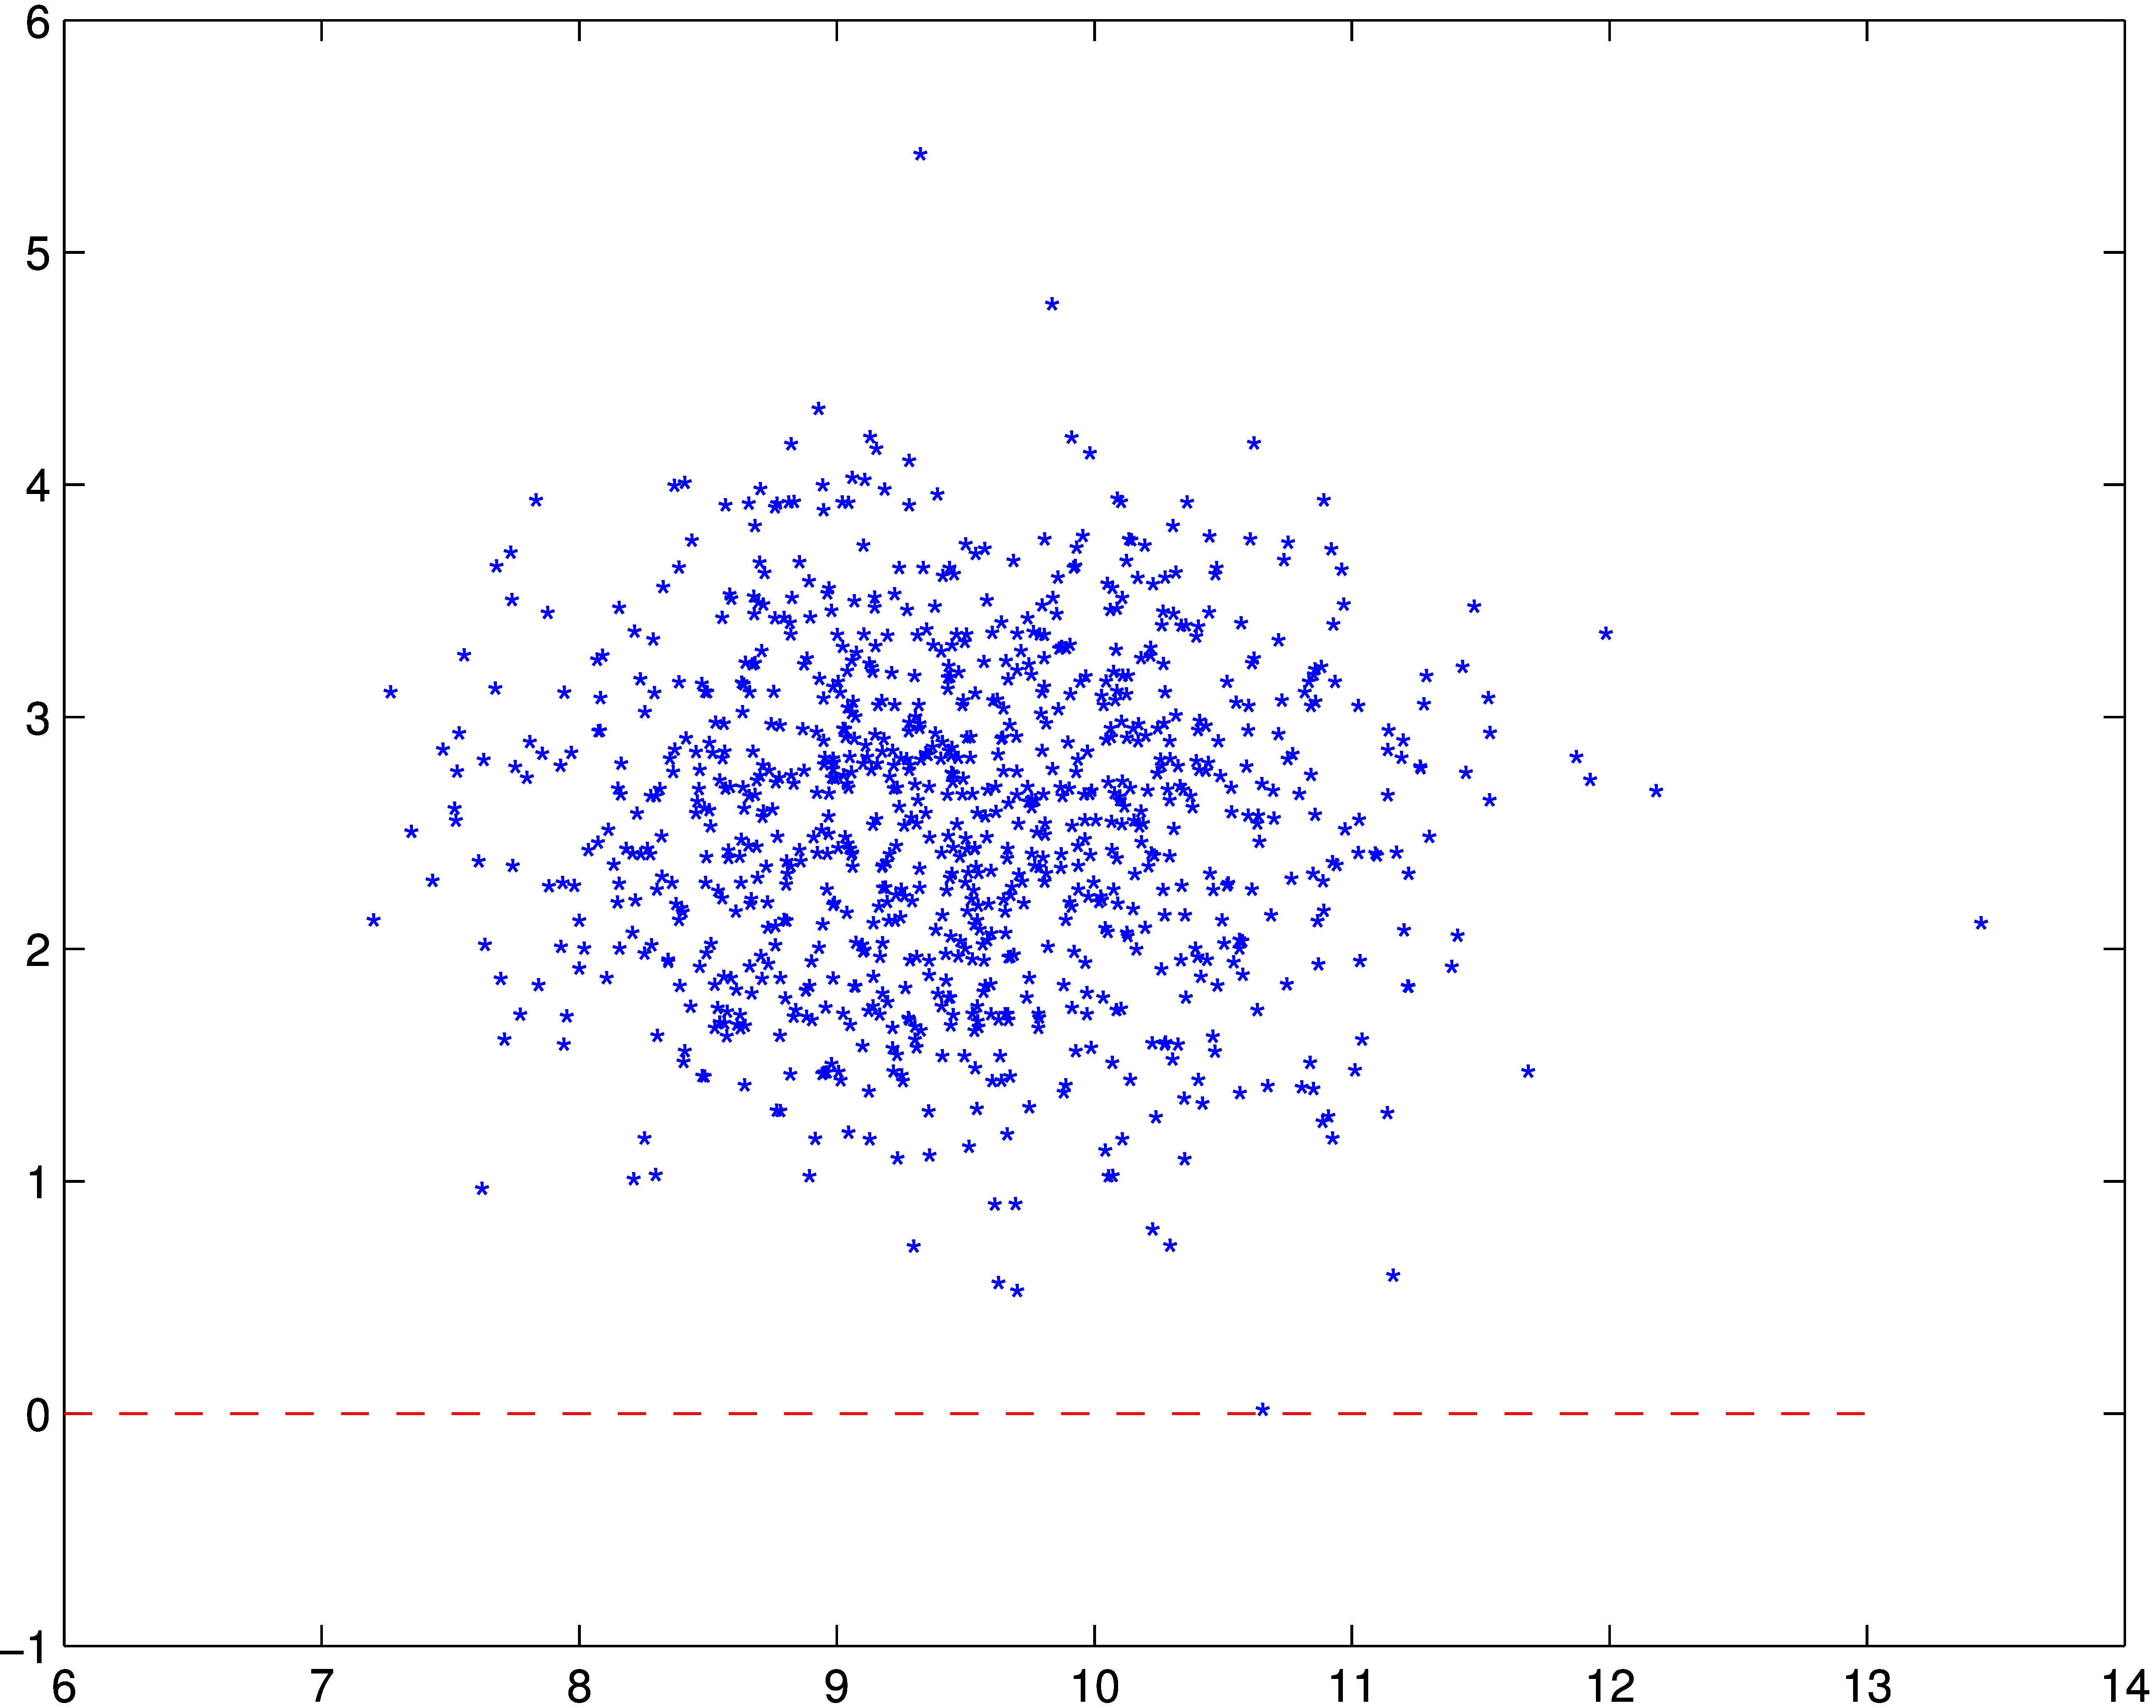
\includegraphics[scale=.8]{pics/taxscat_cropped.jpg}
    \caption{Welfare gains in utils under pareto tax regime by log wealth}
    \label{fig:taxscatter}
\end{figure}
There is a correlation coefficient of $0.179$ between the vindex levels and the pareto taxes presented above.  This is positive, as one might expect, meaning that more visible goods are more heavily taxed.
The mean pre-tax utility level is 92, and the median is 94.  The mean welfare increase in utils is 2.517, and the median increase is 2.547.  The point I want to make in this section is not that these are the actual optimal taxes from a pareto perspective.  Instead I just want to point out that it is easy to generate taxes which benifit all of society and provide large welfare gains.

\section{Conclusion}
This paper takes a conspicuous consumption model from the theory literature seriously by adding preference heterogeneity and estimating parameters from data.
The results of the estimation show that:
\begin{enumerate}
    \item Signaling plays an important role in consumption decisions.  Chinese consumers value peer group belief about well-being more than a third as much as they value direct utility from consumption.
    \item Chinese consumers value signaling more than American consumers.  American consumers value peer group belief about a sixth as much as they value direct utility.
    \item It is easy to find excise taxes which lead to large welfare gains, and do not hurt anyone.
\end{enumerate}
	These results indicate that, in India, a tax on festival spending may significantly increase welfare.
In the United States, I suggest a large tax on Apple products.

In order to get an estimable model, I had to make quite a few unrealistic assumptions.
One's peer group sees only consumption expenditures in one good category. 
This is clearly counterfactual.
In the real world, one's peer group sees a full vector of consumption expenditures, but with some noise.
An earlier version of this paper had a model with this feature, but estimation involved numerically calculating a thirty dimensional integral for each consumer for each parameter trial.
Future research might focus on finding a tractible model to estimate without such a stark assumption about the observability of consumption.
\bibliographystyle{plainnat}
\bibliography{biglist.bib}


\end{document}
